\chapter{Fundamentação Teórica}
\label{cap:fund}

%% - - - - - - - - - - - - - - - - - - - - - - - - - - - - - - - - - - -
\section{Aprendizado por Reforço}
\label{sec:rl}

O Aprendizado por Reforço (\textit{Reinforcement Learning} - RL) é uma abordagem de aprendizado baseada na interação entre um agente e seu ambiente, onde o objetivo principal é maximizar um sinal de recompensa acumulada ao longo do tempo \cite{sutton}. O agente aprende a tomar decisões através de tentativa e erro, ajustando suas ações com base no \textit{feedback} recebido. Diferentemente do aprendizado supervisionado, que utiliza exemplos rotulados, o aprendizado por reforço explora a recompensa como único sinal de desempenho, lidando com a complexidade de recompensas atrasadas e incertezas na transição de estados. Formalmente, o RL é modelado através de \textbf{processos de decisão de Markov} (\textit{Markov Decision Processes} - MDPs) \cite{sutton}, que definem as interações em termos de estados, ações e recompensas, sendo amplamente aplicável a problemas de decisão sequencial em diversas áreas.

Dentre os métodos avançados de aprendizado por reforço, destaca-se o \textbf{\textit{Proximal Policy Optimization} (PPO)} \cite{PPO}, que é amplamente utilizado devido à sua estabilidade em ambientes complexos. Quando aplicado ao \textbf{aprendizado por reforço multiagente} (\textit{Multi-agent RL}), permite que diversos agentes aprendam simultaneamente, interagindo de maneira colaborativa ou competitiva. Estratégias como o \textit{self-play} têm mostrado grande eficácia ao permitir que agentes aprendam uns com os outros em cenários competitivos, como no futebol de robôs. Além disso, o \textit{curriculum learning} \cite{curriculum} tem sido utilizado para estruturar a aprendizagem progressiva, começando com tarefas simples e avançando para desafios mais complexos \cite{curriculum_task_sequence}, um aspecto crucial em domínios como o \textbf{futebol de robôs}, onde os agentes precisam coordenar habilidades motoras e estratégias de equipe para alcançar um bom desempenho.

\subsection{Conceitos Básicos}
\label{subsec:rl_conceitos}

A interação entre o agente e o ambiente é representada esquematicamente na Figura \ref{fig:agent_env_interaction}. O agente observa o estado atual \( S_t \) do ambiente e, com base em sua política de decisão, escolhe uma ação \( A_t \). Após a execução dessa ação, o ambiente evolui para um novo estado \( S_{t+1} \) e retorna ao agente uma recompensa \( R_{t+1} \) associada a essa transição.

\begin{figure}[h]
    \centering
    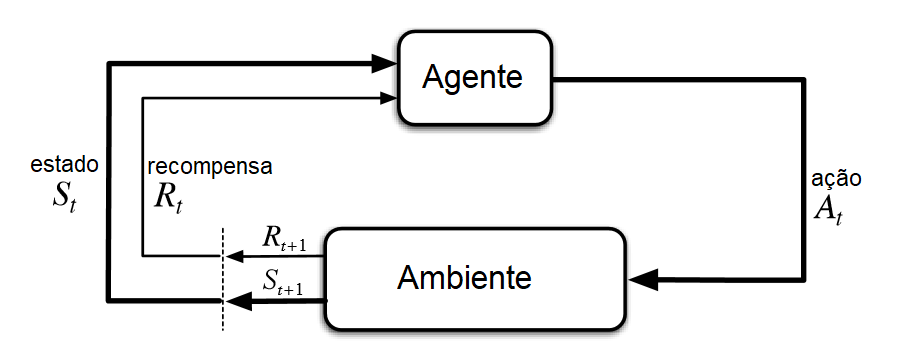
\includegraphics[width=0.6\textwidth]{fig/MDP.png}
    \caption{Interação agente-ambiente no aprendizado por reforço. O agente toma decisões com base no estado atual \( S_t \) e recebe do ambiente uma recompensa \( R_{t+1} \) após realizar a ação \( A_t \).}
    \label{fig:agent_env_interaction}
\end{figure}

\subsubsection*{Elementos Fundamentais:}
\begin{enumerate}
    \item \textbf{Agente e Ambiente:} O agente é a entidade responsável por tomar decisões, enquanto o ambiente é tudo aquilo que responde às ações do agente e fornece \textit{feedback}.
    \item \textbf{Política (\(\pi\)):} Define a estratégia do agente, especificando a probabilidade de selecionar uma ação específica \( A_t \) em um estado \( S_t \).
    \item \textbf{Sinal de Recompensa (\(R_{t+1}\)):} Indica o valor imediato recebido pelo agente após realizar uma ação. O objetivo é maximizar a soma acumulada das recompensas ao longo do tempo.
    \item \textbf{Função de Valor (\(v(s)\) e \(q(s, a)\)):} Estima o valor esperado da recompensa futura a partir de um estado \( s \) ou de um par estado-ação \( (s, a) \).
\end{enumerate}

\subsubsection*{Exploração vs. Intensificação:}
O dilema entre exploração e intensificação é um aspecto fundamental do aprendizado por reforço, especialmente em aprendizado multiagente \cite{PPO}. Em sistemas multiagente, este dilema torna-se complexo devido à não-estacionariedade do ambiente, onde os agentes precisam explorar enquanto se adaptam aos comportamentos em evolução de outros agentes \cite{bruno_brandao}. Técnicas como aprendizado centralizado com execução descentralizada (\textit{Centralized Training with Decentralized Execution} - CTDE) e modelagem de oponentes são empregadas para gerenciar eficientemente este compromisso, permitindo que os agentes compartilhem experiências de exploração enquanto mantêm estratégias eficazes de intensificação \cite{ppo_exploration_exploitation}.

\subsubsection*{Modelagem por Processos de Decisão de Markov (MDPs)}

O aprendizado por reforço é frequentemente modelado por \textbf{Processos de Decisão de Markov} (\textit{Markov Decision Processes} - MDPs) \cite{sutton}, uma estrutura matemática que captura os aspectos estocásticos e sequenciais da tomada de decisão. Um MDP é definido pela quádrupla \((S, A, P, R)\), onde:

\begin{itemize}
    \item \(S\) é o conjunto de estados possíveis do ambiente.
    \item \(A\) é o conjunto de ações possíveis que o agente pode tomar.
    \item \(P(s'|s, a)\) é a distribuição de probabilidade de transição para o estado \(s'\) dado o estado atual \(s\) e a ação \(a\) tomada.
    \item \(R(s, a)\) é a função de recompensa esperada ao tomar a ação \(a\) no estado \(s\).
\end{itemize}

O agente busca maximizar a soma esperada das recompensas acumuladas ao longo do tempo, definida pelo \textbf{retorno} \(G_t\) \cite{sutton}. No caso de problemas de horizonte finito, o retorno é por 

\begin{equation}
\label{eq:retorno_finito}
G_t = \sum_{k=0}^{T} \gamma^k R_{t+k+1}.
\end{equation}

Onde \(\gamma\) é o fator de desconto, que no caso de tarefas contínuas, aplica-se \(\gamma \in [0, 1]\) que controla o peso das recompensas futuras,

\begin{equation}
\label{eq:retorno_infinito}
G_t = R_{t+1} + \gamma R_{t+2} + \gamma^2 R_{t+3} + \dots = \sum_{k=0}^{\infty} \gamma^k R_{t+k+1}.
\end{equation}

A modelagem dos MDPs requer duas funções principais de valor, que capturam a expectativa de recompensas futuras:

\paragraph{1. Função de valor de estado (\(v_\pi(s)\)) \cite{sutton}:}
Define o valor esperado de se estar no estado \(s\) e seguir uma política \(\pi\) a partir desse estado, conforme a Equação 

\begin{equation}
\label{eq:valor_estado}
v_\pi(s) = \mathbb{E}_\pi \left[ \sum_{k=0}^{\infty} \gamma^k R_{t+k+1} \mid S_t = s \right].
\end{equation}

Essa função pode ser definida recursivamente pela \textbf{equação de Bellman}, como mostrado na Equação 

\begin{equation}
\label{eq:bellman_estado}
v_\pi(s) = \sum_{a \in A} \pi(a|s) \sum_{s' \in S} P(s'|s, a) \left[ R(s, a) + \gamma v_\pi(s') \right];
\end{equation}

\paragraph{2. Função de valor de ação (\(q_\pi(s, a)\)) \cite{sutton}:}
Define o valor esperado de se tomar a ação \(a\) no estado \(s\) e seguir a política \(\pi\) posteriormente, como apresentado na Equação 

\begin{equation}
\label{eq:valor_acao}
q_\pi(s, a) = \mathbb{E}_\pi \left[ \sum_{k=0}^{\infty} \gamma^k R_{t+k+1} \mid S_t = s, A_t = a \right].
\end{equation}

Também pode ser escrita de forma recursiva, conforme a Equação 

\begin{equation}
\label{eq:bellman_acao}
q_\pi(s, a) = \sum_{s'} P(s'|s, a) \left[ R(s, a) + \gamma \sum_{a'} \pi(a'|s') q_\pi(s', a') \right].
\end{equation}

\paragraph{Equação de Bellman para o Ótimo \cite{sutton}:}
Para políticas ótimas \(\pi^*\), temos as funções de valor ótimo, dada pela Equação 

\begin{equation}
\label{eq:bellman_otimo_estado}
v^*(s) = \max_a \sum_{s'} P(s'|s, a) \left[ R(s, a) + \gamma v^*(s') \right], 
\end{equation} 
e a função de valor de ação ótima, apresentada na Equação 

\begin{equation}
\label{eq:bellman_otimo_acao}
q^*(s, a) = \sum_{s'} P(s'|s, a) \left[ R(s, a) + \gamma \max_{a'} q^*(s', a') \right].
\end{equation}

Essas equações de Bellman são fundamentais para algoritmos de planejamento, como \textit{Value Iteration} e \textit{Policy Iteration}, mas quando a dinâmica do ambiente não é conhecida, métodos de aprendizado baseados em interação, como \textit{Q-learning}, se tornam necessários.

Os MDPs constituem o núcleo matemático de muitos algoritmos de aprendizado por reforço, e são essenciais para o desenvolvimento de métodos de otimização de políticas, como o \textbf{\textit{Proximal Policy Optimization} (PPO)}. Este algoritmo combina exploração e estabilidade ao ajustar políticas dentro de uma região de confiança definida.

\subsection{PPO (\textit{Proximal Policy Optimization})}
\label{subsec:ppo}

O \textit{Proximal Policy Optimization} (PPO) representa um marco significativo no desenvolvimento de algoritmos de aprendizado por reforço, destacando-se pela sua combinação única de simplicidade de implementação, eficiência computacional e estabilidade durante o treinamento \cite{PPO}. Desenvolvido pela OpenAI, o PPO surgiu como uma evolução do \textit{Trust Region Policy Optimization} (TRPO), introduzindo mecanismos mais eficientes para controlar a magnitude das atualizações de política \cite{openia_ppo_doc}.

O diferencial do PPO está em sua abordagem para otimização de políticas, que utiliza uma \textit{função objetivo substituta recortada} (\textit{clipped surrogate objective}) \cite{PPO, openia_ppo_doc}. Esta função limita efetivamente as mudanças na política, prevenindo atualizações muito grandes que poderiam desestabilizar o aprendizado. Matematicamente, a função objetivo do PPO é expressa como:

\begin{equation}
L^{CLIP}(\theta) = \mathbb{E}_t \left[ \min\left( r_t(\theta) A_t, \text{clip}(r_t(\theta), 1-\epsilon, 1+\epsilon) A_t \right) \right],
\end{equation}
onde $r_t(\theta) = \frac{\pi_\theta(a_t|s_t)}{\pi_{\theta_{old}}(a_t|s_t)}$ representa a razão entre as probabilidades das políticas nova e antiga, $A_t$ é a estimativa da vantagem, e $\epsilon$ é um hiperparâmetro que controla o tamanho máximo da atualização \cite{stable_baselines3, PPO}.

O PPO implementa uma arquitetura \textit{actor-critic}, onde o \textit{actor} é responsável pela política que mapeia estados para ações, enquanto o \textit{critic} estima os valores dos estados para auxiliar no cálculo das vantagens \cite{PPO, pytorch_ppo}. Esta estrutura dual permite um equilíbrio eficiente entre exploração e aproveitamento do conhecimento adquirido. O processo de treinamento ocorre em episódios, onde experiências são coletadas e utilizadas para atualizar tanto a política quanto a função de valor \cite{PPO}.

Uma característica fundamental do PPO é sua capacidade de lidar com espaços de ação tanto discretos quanto contínuos, tornando-o particularmente adequado para aplicações em robótica e controle \cite{sutton, PPO}. O algoritmo mantém um equilíbrio entre exploração e exploração através de um termo de entropia adicional na função objetivo, que incentiva a política a manter um nível apropriado de aleatoriedade nas decisões \cite{PPO}.

O PPO tem demonstrado resultados impressionantes em uma variedade de domínios complexos, desde jogos até tarefas de robótica \cite{ppo_env_gym}. Sua eficácia é particularmente notável em ambientes que requerem aprendizado contínuo e adaptação, como no caso do futebol de robôs, onde os agentes precisam constantemente ajustar suas estratégias em resposta a situações dinâmicas \cite{bruno_brandao}.

No contexto do aprendizado multiagente, o PPO pode ser estendido para treinar múltiplos agentes simultaneamente, permitindo o desenvolvimento de comportamentos cooperativos ou competitivos \cite{pytorch_ppo}. Esta característica é especialmente relevante para cenários de equipe, como o futebol de robôs, onde os agentes precisam coordenar suas ações para alcançar objetivos comuns \cite{ppo_env_gym, bruno_brandao}.

\subsection{Multi-agent RL}
\label{subsec:marl}

O Aprendizado por Reforço Multiagente (\textit{Multi-agent Reinforcement Learning} - MARL) representa uma extensão fundamental do RL tradicional, onde múltiplos agentes autônomos interagem em um ambiente compartilhado, aprendendo simultaneamente através de suas experiências coletivas. Como destacado em \cite{bruno_brandao}, esta abordagem expande o paradigma clássico dos Processos de Decisão Markovianos (MDPs) para acomodar as complexidades inerentes às interações entre múltiplos tomadores de decisão.

A transição do RL \textit{single-agent} para o MARL introduz desafios significativos, principalmente relacionados à não-estacionariedade do ambiente. Como observado em \cite{seac_multiagent}, quando múltiplos agentes atualizam suas políticas simultaneamente, o ambiente torna-se não-estacionário do ponto de vista de cada agente individual, violando premissas fundamentais do RL tradicional. Esta característica exige o desenvolvimento de algoritmos especializados que possam lidar com a natureza dinâmica das interações multiagente.

Um aspecto crucial do MARL, conforme destacado em \cite{review_cooperative_multi_agent}, é a distinção entre cenários cooperativos e competitivos. Em ambientes cooperativos, os agentes trabalham juntos para maximizar uma recompensa global compartilhada, enquanto em cenários competitivos, cada agente busca otimizar sua própria recompensa, potencialmente em detrimento dos outros.

A escalabilidade representa outro desafio significativo no MARL. De acordo com \cite{efficient_multi_agent}, o espaço de ações conjunto cresce exponencialmente com o número de agentes, tornando necessário o desenvolvimento de técnicas de decomposição e aproximação. Abordagens recentes, como o MAZero, têm demonstrado sucesso ao combinar planejamento baseado em modelo com técnicas de busca em árvore \textit{Monte Carlo} para navegar eficientemente por estes espaços complexos.

Para lidar com estes desafios, diversas arquiteturas e algoritmos têm sido propostos. \cite{agentes_inteligentes_puc} destaca a importância de métodos como QMIX e MADDPG, que utilizam estruturas de valor decompostas e críticos centralizados para facilitar o aprendizado em ambientes multiagente. Estas abordagens permitem o treinamento centralizado com execução descentralizada, um paradigma que tem se mostrado particularmente eficaz em aplicações práticas.

A aplicação do MARL em domínios reais tem demonstrado resultados promissores. Como evidenciado em \cite{martins_vss}, no contexto do futebol de robôs, abordagens multiagente superam significativamente métodos \textit{single-agent}, especialmente em cenários que exigem coordenação complexa entre os membros da equipe. No entanto, o sucesso destas aplicações depende crucialmente da modelagem adequada das funções de recompensa e da implementação de mecanismos eficientes de comunicação entre agentes.

Desenvolvimentos recentes no campo, como destacado em \cite{survey_multi_agent}, têm explorado a integração do MARL com outras tecnologias emergentes, como grandes modelos de linguagem e técnicas de aprendizado por demonstração. Estas integrações abrem novos caminhos para o desenvolvimento de sistemas multiagente mais sofisticados e adaptáveis, capazes de lidar com tarefas cada vez mais complexas em ambientes dinâmicos.

\subsection{\textit{Self-play}}
\label{subsec:self_play}

O \textit{Self-play} emergiu como uma técnica fundamental no aprendizado por reforço, permitindo que agentes artificiais desenvolvam habilidades avançadas através do treinamento contra versões de si mesmos. Como destacado em \cite{survey_self_play}, esta abordagem permite que os agentes criem um currículo automático de aprendizado, onde enfrentam adversários progressivamente mais desafiadores, evitando assim a estagnação em estratégias subótimas.

A eficácia do \textit{self-play} foi demonstrada de forma notável em diversos domínios complexos. Conforme documentado em \cite{alpha_zero}, sistemas como AlphaGo e AlphaZero alcançaram desempenho sobre-humano em jogos estratégicos complexos, aprendendo exclusivamente através da interação consigo mesmos.

Um aspecto crucial do \textit{self-play}, como apontado em \cite{survey_self_play_2024}, é sua capacidade de gerar dados de treinamento de alta qualidade sem necessidade de supervisão humana. Esta característica é particularmente valiosa em domínios onde exemplos de especialistas são escassos ou caros de obter. O processo permite que os agentes explorem o espaço de estratégias de forma mais abrangente do que seria possível com dados puramente supervisionados.

A implementação moderna do \textit{self-play} frequentemente incorpora arquiteturas sofisticadas. De acordo com \cite{self_play_adversarial_critic}, o método SPAC (\textit{Self-Play Actor-Critic}) introduziu inovações significativas ao integrar um crítico que considera as observações de ambos os agentes em ambientes competitivos, superando métodos tradicionais em eficácia.

No entanto, o \textit{self-play} também apresenta desafios significativos. Como observado em \cite{provable_self_play}, existe o risco de convergência para equilíbrios subótimos, especialmente em jogos com múltiplos equilíbrios de Nash. Para mitigar este problema, técnicas como diversificação de oponentes e regularização de entropia têm sido empregadas com sucesso.

Desenvolvimentos recentes, descritos em \cite{survey_self_play, survey_self_play_2024}, têm explorado a integração do \textit{self-play} com paradigmas emergentes como meta-aprendizado e modelos de linguagem grandes. Esta convergência tem aberto novos caminhos para o desenvolvimento de agentes mais adaptativos e versáteis.

A aplicação do \textit{self-play} estende-se além dos jogos tradicionais. Como documentado em \cite{survey_self_play_2024} e \cite{bruno_brandao}, a técnica tem sido aplicada com sucesso em domínios como robótica, simulações financeiras e sistemas de controle autônomo. Em cada caso, o \textit{self-play} permite que os agentes desenvolvam estratégias robustas através da exploração sistemática do espaço de possibilidades.

O futuro do \textit{self-play} parece promissor, com pesquisas contínuas focando na melhoria da eficiência computacional e na expansão de suas aplicações. Como sugerido em \cite{huggingface_self_play}, novas técnicas de otimização e paralelização estão tornando o treinamento mais acessível, permitindo sua aplicação em uma gama cada vez maior de problemas práticos.

%% - - - - - - - - - - - - - - - - - - - - - - - - - - - - - - - - - - -
\section{\textit{Curriculum Learning}}
\label{sec:curriculum}

O \textit{Curriculum Learning} (CL) representa uma abordagem metodológica inspirada nos princípios pedagógicos humanos, onde o processo de aprendizagem é estruturado de forma progressiva, começando com tarefas mais simples e avançando gradualmente para desafios mais complexos. Esta metodologia tem demonstrado resultados significativos na otimização do treinamento de agentes de aprendizado, especialmente em contextos de \textit{Reinforcement Learning} (RL), como destacado por \cite{curriculum_learning_a_survey}.

\subsection{Conceitos Fundamentais}
\label{subsec:curriculum_conceitos}

O \textit{Curriculum Learning} fundamenta-se em três componentes principais que trabalham em conjunto para estruturar o processo de aprendizagem. Como descrito em \cite{curriculum}, estes componentes são: geração de tarefas, sequenciamento e transferência de conhecimento.

A geração de tarefas envolve a criação sistemática de desafios intermediários que estabelecem uma ponte entre o estado inicial do agente e o objetivo final desejado. De acordo com \cite{curriculum_reinforcement_learning}, este processo pode incluir a modificação controlada de parâmetros ambientais, como a densidade de recompensas ou a complexidade dos estados apresentados ao agente.

O sequenciamento, por sua vez, representa a ordenação estratégica das tarefas geradas, garantindo uma progressão coerente e efetiva no processo de aprendizagem. Como destacado em \cite{curriculum}, esta ordenação pode ser realizada através de métodos como Interpolação de Distribuições ou \textit{Optimal Transport}, que otimizam a trajetória de aprendizado do agente.

A transferência de conhecimento, elemento crucial do CL, permite que o aprendizado adquirido em tarefas anteriores seja efetivamente utilizado para acelerar o domínio de novos desafios. \cite{diffusion_based_curriculum_reinforcement_learning} demonstra que técnicas como o \textit{Boosted Curriculum RL} (BCRL) podem aproximar funções de valor como somas de resíduos treinados incrementalmente, aumentando significativamente a capacidade expressiva do modelo.

Um aspecto fundamental do CL, conforme apresentado por \cite{curriculum}, é a utilização de métricas de dificuldade para calibrar a progressão do currículo. Estas métricas podem incluir a entropia das políticas aprendidas ou a taxa de sucesso em submetas específicas, permitindo um ajuste dinâmico do processo de aprendizagem.

No contexto específico do \textit{Reinforcement Learning}, o CL se integra naturalmente com os Processos de Decisão de Markov (MDPs), onde o agente interage com ambientes parametrizados de forma progressiva \cite{sutton}. Esta integração, como explicado em \cite{curriculum_reinforcement_learning}, permite uma acumulação estruturada de experiência, fundamental para o desenvolvimento de políticas robustas e eficientes.

\subsection{Aplicações em RL}
\label{subsec:curriculum_rl}

No contexto do \textit{Reinforcement Learning}, o \textit{Curriculum Learning} tem se mostrado particularmente eficaz em cenários complexos que apresentam desafios significativos para métodos tradicionais de aprendizagem. Como destacado por \cite{curriculum_reinforcement_learning}, a aplicação de currículos estruturados tem permitido avanços notáveis em domínios que exigem raciocínio hierárquico e planejamento de longo prazo.

Um exemplo significativo é encontrado em ambientes de navegação autônoma, onde \cite{automatic_curriculum_learning_survey, huggingface_curriculum} demonstra que agentes treinados com CL desenvolvem estratégias mais robustas ao serem expostos gradualmente a ambientes de complexidade crescente. O processo começa com cenários simplificados, como navegação em espaços abertos, e progride para ambientes com obstáculos dinâmicos e restrições temporais, resultando em políticas mais generalizáveis.

Em aplicações de robótica, \cite{curriculum} apresenta uma abordagem onde o CL é utilizado para decompor tarefas motoras complexas em subcomponentes mais gerenciáveis. Os autores demonstram que esta decomposição hierárquica não apenas acelera o aprendizado, mas também melhora significativamente a qualidade das políticas aprendidas, especialmente em tarefas que requerem coordenação motora fina.

A integração do CL com técnicas de aprendizado multiagente tem produzido resultados promissores, como evidenciado por \cite{curriculum_learning_in_rl}. Em cenários competitivos e cooperativos, o uso de currículos adaptativos permite que os agentes desenvolvam estratégias sofisticadas através da exposição gradual a adversários ou parceiros de diferentes níveis de habilidade. Esta abordagem tem se mostrado particularmente eficaz em domínios como o futebol de robôs, onde a complexidade das interações entre agentes pode tornar o aprendizado direto impraticável.

Um aspecto crucial na aplicação do CL em RL, conforme destacado por \cite{variational_curriculum_rl}, é a capacidade de automatizar a geração e adaptação de currículos. Técnicas recentes utilizam meta-aprendizado para otimizar a sequência de tarefas, permitindo que o currículo se ajuste dinamicamente ao progresso do agente. Esta automatização não apenas reduz a necessidade de intervenção humana, mas também permite a descoberta de sequências de treinamento não intuitivas que podem levar a um melhor desempenho.

A eficácia do CL em RL também se estende a domínios com espaços de estado contínuos e de alta dimensionalidade. \cite{curml} demonstra como currículos bem projetados podem guiar a exploração em espaços complexos, reduzindo significativamente o tempo necessário para encontrar políticas ótimas. Esta abordagem tem se mostrado particularmente valiosa em aplicações industriais, onde o custo de exploração aleatória pode ser proibitivo.

Diversos avanços significativos têm sido feitos na área de \textit{Curriculum Learning}, incluindo automatização do design de currículos, integração com aprendizado profundo, \textit{frameworks} baseados em modelos de difusão para geração automática de tarefas, coordenação de currículos paralelos em sistemas multiagente e desenvolvimento de currículos auto-adaptativos baseados em meta-aprendizado \cite{curriculum_reinforcement_learning, diffusion_based_curriculum_reinforcement_learning, curriculum_learning_in_rl, variational_curriculum_rl}. Estas inovações têm contribuido para melhorar a forma como os currículos são estruturados e aplicados, permitindo uma evolução significativa na área.

\subsection{Vantagens e desafios}
\label{subsec:curriculum_vantagens_desafios}

A implementação do \textit{Curriculum Learning} apresenta tanto benefícios substanciais quanto desafios significativos que precisam ser cuidadosamente considerados. Como observado por \cite{curriculum_learning_in_rl}, as vantagens incluem uma aceleração significativa no processo de aprendizagem e uma melhoria na qualidade das políticas aprendidas.

Entre as principais vantagens, \cite{curriculum_reinforcement_learning} destaca a redução significativa no tempo de treinamento, com alguns experimentos mostrando uma diminuição de até 60\% no número de iterações necessárias para convergência. Além disso, os autores observam uma melhoria na robustez das políticas aprendidas, com agentes demonstrando maior capacidade de generalização para cenários não vistos durante o treinamento.

No entanto, existem desafios importantes a serem considerados. Como apontado por \cite{boosted_curriculum_rl}, um dos principais obstáculos é a definição apropriada de métricas de dificuldade para diferentes tipos de tarefas. A subjetividade inerente à noção de "dificuldade" pode tornar complexa a automatização completa do processo de \textit{design} do currículo.

 \cite{curriculum} identifica outro desafio significativo: o balanceamento entre exploração e exploração durante o processo de aprendizagem. Currículos mal calibrados podem levar a uma convergência prematura para soluções subótimas ou, alternativamente, resultar em uma exploração excessiva que compromete a eficiência do treinamento.

Um aspecto particularmente desafiador, conforme destacado por \cite{curml}, é a necessidade de recursos computacionais significativos para a implementação efetiva de currículos adaptativos. O custo de gerar e validar sequências de treinamento personalizadas pode ser proibitivo para algumas aplicações, especialmente em domínios que requerem simulações complexas ou processamento em tempo real.

Apesar destes desafios, na literatura, como evidenciado por \cite{curriculum_learning_a_survey}, a expextativa é que os benefícios do \textit{Curriculum Learning} geralmente superam suas limitações, especialmente em domínios complexos onde abordagens tradicionais de aprendizado por reforço mostram-se inadequadas. A contínua evolução de técnicas automatizadas para \textit{design} de currículos e a crescente disponibilidade de recursos computacionais sugerem um futuro promissor para esta abordagem.

%% - - - - - - - - - - - - - - - - - - - - - - - - - - - - - - - - - - -
\section{Futebol de Robôs}
\label{sec:futebol_robos}

O futebol de robôs representa uma das principais plataformas para pesquisa e desenvolvimento em robótica móvel e sistemas multiagentes. Dentro deste contexto, a \textit{RoboCup Small Size League Entry Level} (SSL-EL) emerge como uma categoria especialmente projetada para facilitar a entrada de novas equipes, mantendo os desafios técnicos fundamentais do futebol de robôs enquanto simplifica aspectos complexos da competição \cite{regras_ssl_el_2024}.

\subsection{Visão geral}
\label{subsec:futebol_visao}

A SSL-EL foi estabelecida como uma divisão de entrada da \textit{Small Size League}, visando democratizar o acesso à competição de futebol de robôs. Diferentemente da divisão principal, a SSL-EL opera com 6 robôs por equipe em um campo reduzido, permitindo que equipes iniciantes desenvolvam suas habilidades técnicas e estratégicas de forma progressiva \cite{regras_ssl_el_2024}.

O ambiente de jogo é estruturado em torno de um sistema centralizado de visão (\textit{SSL-Vision}), que fornece informações em tempo real sobre as posições dos robôs e da bola através de câmeras suspensas \cite{ssl_overview}. Esta arquitetura permite que as equipes foquem no desenvolvimento de estratégias de controle e coordenação, sem a necessidade inicial de implementar sistemas complexos de percepção local.

Os robôs da SSL-EL, embora sujeitos a restrições dimensionais similares às da divisão principal (diâmetro $\leq 18$ cm, altura $\leq 15$ cm) \cite{regras_ssl_el_2024}, podem ser construídos com soluções mais acessíveis. A equipe \textit{TurtleRabbit}, por exemplo, demonstrou a viabilidade de construir robôs competitivos com orçamento reduzido, utilizando componentes comerciais e estruturas impressas em 3D \cite{turtlerabbit_tdp_2024}.

A competição promove desafios técnicos específicos, como o \textit{Ball Placement Challenge}, que permitem às equipes desenvolverem e testarem capacidades fundamentais de forma isolada \cite{ssl_overview}. Esta abordagem gradual ao desenvolvimento de habilidades tem se mostrado efetiva para a evolução das equipes, como evidenciado pelos resultados de competições recentes \cite{ssl_overview}.

\subsection{Desafios específicos}
\label{subsec:futebol_desafios}

A SSL-EL apresenta desafios únicos que equilibram complexidade técnica com acessibilidade. Um dos principais desafios é a coordenação multiagente em tempo real, onde os robôs devem operar de forma sincronizada em velocidades consideráveis, tomando decisões em milissegundos \cite{regras_ssl_el_2024}. Esta coordenação torna-se ainda mais complexa devido aos ruídos de percepção e latência de comunicação inerentes ao sistema.

O aspecto financeiro representa outro desafio significativo para equipes iniciantes. No entanto, iniciativas como a da equipe \textit{TurtleRabbit} demonstram que é possível desenvolver soluções competitivas com orçamento limitado \cite{turtlerabbit_tdp_2024}. Através do uso de componentes comerciais acessíveis e técnicas de manufatura como impressão 3D, equipes podem construir robôs funcionais mantendo os custos controlados.

O processamento em tempo real das informações do \textit{SSL-Vision} apresenta desafios técnicos específicos \cite{ssl_overview}. As equipes precisam desenvolver sistemas robustos para lidar com:
- Fusão de dados de múltiplas câmeras
- Compensação de falhas momentâneas na detecção
- Filtragem de ruídos e correção de discrepâncias
- Predição de movimentos para compensar latências

A implementação de estratégias de jogo efetivas também representa um desafio significativo. Como documentado pela equipe \textit{RoboCIn} \cite{robocin_tdp_2024}, é necessário desenvolver algoritmos sofisticados para navegação, controle de bola e coordenação tática, mesmo no contexto simplificado da SSL-EL.

\subsection{Trabalhos relacionados}
\label{subsec:futebol_trabalhos}

Diversos trabalhos têm contribuído para o avanço da SSL-EL, focando em diferentes aspectos da competição. As equipes \textit{ITAndroinds} e \textit{OrcaBOT}, por exemplo, desenvolveu uma abordagem inovadora para o \textit{design} de robôs de baixo custo, documentada em seu \textit{TDP} (\textit{Team Description Paper}) \cite{orcabot_tdp_2024, itandroids_tdp_2023}, demonstrando a viabilidade de construir sistemas competitivos com recursos limitados.

No campo do controle e estratégia, trabalhos significativos têm emergido da comunidade acadêmica \cite{bruno_brandao, robocin_trabalho}. Estas pesquisas demonstram o potencial de algoritmos de aprendizado de máquina para desenvolver estratégias de jogo mais sofisticadas.

A organização da \textit{RoboCup} tem contribuído significativamente através da documentação e padronização de regras e especificações técnicas \cite{regras_ssl_el_2024}. Este trabalho de documentação tem sido fundamental para permitir que novas equipes ingressem na competição com uma compreensão clara dos requisitos e desafios.

Iniciativas de código aberto, como as disponibilizadas pela comunidade brasileira de robótica \cite{robocup_ssl_brasil}, têm facilitado o desenvolvimento de novas equipes. Estes recursos incluem implementações de referência para sistemas de controle, simuladores e ferramentas de desenvolvimento, permitindo que equipes iniciantes construam sobre uma base sólida de conhecimento estabelecido.